% =============================================================================
%  Moroccan Legal Q&A System based on RAG with Arabic NLP
%  Springer LNCS proceedings format  (splnproc2510 / llncs class)
%
%  Compile (command line):
%      pdflatex main
%      bibtex   main
%      pdflatex main
%      pdflatex main
%
%  Or: upload this whole folder to Overleaf (www.overleaf.com) and compile
%  with the default pdfLaTeX engine -- the llncs.cls and splncs04.bst files
%  are already included.
%
%  NOTE: Replace the placeholder authors / affiliation / email below with the
%  actual ICCT2026 submission metadata before final submission.
% =============================================================================

\documentclass[runningheads]{llncs}

% --- Packages ---------------------------------------------------------------
\usepackage[T1]{fontenc}
\usepackage[utf8]{inputenc}
\usepackage{graphicx}
\usepackage{booktabs}
\usepackage{amsmath}
\usepackage{amssymb}
\usepackage{url}
\usepackage{array}
\usepackage{multirow}

\begin{document}

% --- Title -------------------------------------------------------------------
\title{Moroccan Legal Question Answering System Based on Retrieval-Augmented
Generation (RAG) with Arabic Natural Language Processing}
% \titlerunning{Moroccan Legal QA System Based on RAG}  % optional short title

% --- Authors (REPLACE with the real ICCT2026 authors) ------------------------
\author{Author One\orcidID{0000-0000-0000-0000}
        \and
        Author Two\orcidID{0000-0000-0000-0000}
        \and
        Author Three\orcidID{0000-0000-0000-0000}}
\authorrunning{Author One et al.}

\institute{Faculty of Sciences and Techniques of Tangier,
           Abdelmalek Essaadi University, Morocco\\
           \email{firstname.lastname@etu.uae.ac.ma}}

\maketitle

% --- Abstract ----------------------------------------------------------------
\begin{abstract}
This paper presents the design, implementation, and evaluation of a legal
Question Answering (Q\&A) system specialized in Moroccan law, based on the
Retrieval-Augmented Generation (RAG) architecture. The system integrates a
complete Arabic NLP pipeline including text extraction from PDF documents
(digital and scanned), cleaning, Arabic normalization, structural analysis of
legal articles, and vector indexing via PostgreSQL with the pgvector
extension. Hybrid search combines dense cosine similarity (BAAI/bge-m3, 1024
dimensions) with BM25 lexical search, fused through Reciprocal Rank Fusion
(RRF). The generation module relies on Google's Gemma 4 2B model, served on
GPU via Google Colab and exposed through a Cloudflare tunnel. Benchmarks show
that the RRF strategy achieves a Hit@5 of 68.75\% and a Recall@5 of 59.38\%,
while dense search offers the best MRR@5 (0.565). Embedding-model evaluation
demonstrates the superiority of 1024-dimension models
(\texttt{intfloat/multilingual-e5-large}, \texttt{BAAI/bge-m3}) for Arabic
legal text, with domain accuracy reaching 89\%. This work constitutes the
first complete open-source Moroccan legal RAG platform, covering seven areas
of law (criminal, traffic, family, civil, commercial, judicial, tax).
\end{abstract}

\keywords{RAG \and Arabic NLP \and Moroccan Law \and Hybrid Search \and
Multilingual Embeddings \and pgvector \and Gemma 4 \and Legal Question
Answering \and Reciprocal Rank Fusion}

% --- Body --------------------------------------------------------------------
\section{Introduction}
\label{sec:introduction}

Access to legal information is a fundamental right in any state governed by
the rule of law. In Morocco, the legal corpus is vast and complex, comprising
hundreds of laws, codes, and decrees written primarily in Modern Standard
Arabic (MSA). For citizens, legal practitioners, and researchers, navigating
this corpus to find a precise answer to a specific question constitutes a
major challenge. General-purpose search engines (Google, Bing) are poorly
suited to this task: they neither understand the specificity of Arabic legal
vocabulary nor the hierarchical structure of legal codes (articles, chapters,
sections).

Recent advances in Natural Language Processing (NLP), particularly in Large
Language Models (LLMs) and Retrieval-Augmented Generation (RAG)
\cite{lewis2020retrieval}, offer an unprecedented opportunity to build
specialized Question Answering (Q\&A) systems. The RAG approach combines an
information-retrieval module with a text-generation module (LLM), producing
contextualized, sourced, and up-to-date responses without requiring expensive
fine-tuning. However, applying RAG to the Arabic legal domain presents unique
challenges: the scarcity of multilingual embedding models optimized for legal
vocabulary, the morphological complexity of Arabic \cite{habash2010arabic},
the presence of Darija (the Moroccan Arabic dialect) in user queries, the
need for absolute fidelity to legal texts, and the difficulty of processing
scanned historical legal documents.

Our system relies on a corpus of \textbf{2{,}357 legal articles} covering
seven areas of Moroccan law: criminal (822 articles), traffic (228), civil
(705), commercial (359), judicial organization (32), tax (211), and
violations. These articles are extracted from their source PDFs, cleaned,
normalized to standard Arabic, structured with hierarchical metadata, and
indexed in PostgreSQL + pgvector using the
\texttt{intfloat/multilingual-e5-large} embedding model (1024 dimensions).

Our contributions are fourfold:
\begin{enumerate}
  \item A \textbf{complete Arabic NLP processing chain} from PDF extraction
        (digital and scanned) to morphological normalization, cleaning, and
        structural analysis of Moroccan legal codes.
  \item A \textbf{hybrid search architecture} combining dense vector
        similarity (\texttt{BAAI/bge-m3}, 1024 dimensions) with BM25 lexical
        search, fused via Reciprocal Rank Fusion (RRF), indexed in
        PostgreSQL + pgvector with an HNSW index.
  \item A \textbf{systematic benchmark} of five multilingual embedding models
        on 26 Arabic legal articles with 65 query variants covering formal
        Arabic, Darija, French, English, and short/long queries.
  \item A \textbf{comparative benchmark} of three search strategies (dense,
        BM25, RRF) on 32 questions across 7 legal domains, evaluating both
        retrieval quality and generated-answer quality.
\end{enumerate}

The remainder of this paper is organized as follows. Section~\ref{sec:related}
presents related work. Section~\ref{sec:methodology} describes our
methodology. Section~\ref{sec:solution} details the proposed system
architecture. Section~\ref{sec:results} presents experimental results.
Section~\ref{sec:discussion} discusses implications and limitations.
Section~\ref{sec:conclusion} concludes the paper.

\section{Related Work}
\label{sec:related}

The application of NLP to the legal domain has attracted growing interest in
recent years. This section examines existing work in three areas: legal Q\&A
and RAG systems, Arabic language models and embeddings, and hybrid search
strategies.

\subsection{Legal RAG and Q\&A Systems}

The RAG architecture, introduced by Lewis et al.~\cite{lewis2020retrieval},
combines a retriever (typically Dense Passage
Retrieval~\cite{karpukhin2020dense}) with a sequence generator to produce
contextualized responses. Since then, several
specialized RAG systems have emerged in the legal domain.
Louis et al.~\cite{louis2023legal} present Legal-RAG for Indian law using
multilingual embeddings and a fine-tuned LLM, achieving 72\% accuracy on
Indian legal queries. Nguyen et al.~\cite{nguyen2023vietnamese} develop a
similar system for Vietnamese law, demonstrating the importance of linguistic
and cultural adaptation. Closer to our context,
Alshareef et al.~\cite{alshareef2023arabic} propose a Q\&A system for Saudi
law using AraBERT and Elasticsearch for lexical search, achieving 68\%
accuracy on 100 Arabic legal questions. Elaraby et al.~\cite{elaraby2024legal}
present a RAG system for Egyptian law with multilingual embeddings and a
remote LLM. Sharma et al.~\cite{sharma2024indian} propose an Indian Legal RAG
with hybrid search, while Huang et al.~\cite{huang2024sail} present
SAIL-Legal for Chinese law with distributed vector indexing.
Zhou et al.~\cite{zhou2023lexgpt} develop LexGPT, a GPT-4-based legal
assistant with retrieval augmentation. In parallel, domain-adapted pre-trained
language models such as LEGAL-BERT~\cite{chalkidis2020legal} demonstrated
that legal-specific representations outperform generic language models on
legal tasks. Our work extends these approaches by proposing a complete
architecture with advanced hybrid search and systematic benchmarking on
Moroccan law.

\subsection{Arabic NLP for the Legal Domain}

Arabic NLP presents well-documented challenges \cite{habash2010arabic}. The
rich derivational morphology (triliteral roots, patterns, affixes), diglossia
(MSA vs.\ dialects), and ambiguous orthography (alef variants, tatweel,
ligatures) make linguistic preprocessing crucial. In the legal domain
specifically, Zaghouani~\cite{zaghouani2021arabic} highlights the complexity
of Arabic legal vocabulary, characterized by fixed formulas, French and
English borrowings, and elaborate syntax. Benali and
Alami~\cite{benali2025moroccan} note that Moroccan legal Arabic systems must
handle very long sentences (often over 100 words per article), a high degree
of co-reference, non-standard abbreviations, and frequent Arabic--French
code-switching. Nassif et al.~\cite{nassif2024arabic} provide a comprehensive
survey of recent Arabic NLP advances, confirming that rich morphology and
diglossia remain open challenges. Tools such as the CAMeL Tools
suite~\cite{obaraj2021cameltools} offer morphological analyzers for standard
Arabic, though their application to legal text requires adaptation.

\subsection{Multilingual Embedding Models}

Embedding-model choice is crucial in any RAG system. For Arabic,
Ali et al.~\cite{ali2022arabic} compare LaBSE, XLM-R, and AraBERT, concluding
that LaBSE~\cite{feng2022labse} offers the best cross-lingual performance.
Distillation-based approaches~\cite{reimers2020multilingual} further extend
monolingual embeddings to hundreds of languages. Wang et al.%
\cite{wang2023bge} introduce BGE-M3, a multi-granularity model supporting
100+ languages. Liang et al.~\cite{liang2023multilingual} present E5-large,
based on contrastive pre-training. Both BGE-M3 and E5-large produce
1024-dimension embeddings, offering superior representational capacity over
768-dimension models. Our benchmark (Section~\ref{sec:results}) is, to the
best of our knowledge, the first to systematically compare these five models
on Arabic legal text with multilingual query variants.

\subsection{Hybrid Search Strategies}

Dense (vector) search captures semantic similarity but may miss exact lexical
matches. BM25 excels at exact matching but ignores semantic context
\cite{robertson2009bm25}. Transformer-based rankers~\cite{lin2021hybrid}
bridge this gap but are computationally expensive at scale. Reciprocal Rank
Fusion (RRF)~\cite{cormack2009reciprocal}
is a parameter-free fusion method that combines rankings from multiple
systems. Shao et al.~\cite{shao2023hybrid} demonstrate that hybrid
Dense + BM25 + RRF offers the best results for legal queries. Our benchmark
confirms these findings in the Arabic legal domain, with Hit@5 improving from
65.62\% (dense) to 68.75\% (RRF).

\subsection{Large Language Models for Arabic}

Gemma 4~\cite{google2025gemma4} is Google's fourth-generation open model,
available in 2B and 9B sizes, supporting Arabic with competitive performance.
Our system uses Gemma 4 2B in Q4\_K\_XL quantization via
llama.cpp~\cite{gerganov2023llamacpp}. Recent studies~\cite{hendy2023llm} show
that multilingual LLMs can correctly answer Arabic legal questions without
specific fine-tuning, provided they receive relevant context via RAG.

\subsection{Comparative Synthesis}

Table~\ref{tab:related_synthesis} summarizes the technical characteristics of
recent legal RAG systems compared with our proposal.

\begin{table}[t]
\centering
\caption{Comparative synthesis of recent legal RAG systems.}
\label{tab:related_synthesis}
\small
\begin{tabular}{@{}lllll@{}}
\toprule
\textbf{System} & \textbf{Domain} & \textbf{Search} & \textbf{Embedding} & \textbf{Best} \\
\midrule
Lewis et al.\ (2020)  & General   & DPR             & BERT     & 68\% (R@20) \\
Louis et al.\ (2023)  & Indian    & Dense (FAISS)   & E5       & 72\% (P@1) \\
Alshareef et al.\ (2023) & Saudi & Lexical (ES)   & AraBERT  & 68\% (Acc.) \\
Zhou et al.\ (2023)   & US         & Hybrid (GPT-4)  & Ada-002  & N/D \\
Nguyen et al.\ (2023) & Vietnamese & Dense (FAISS) & PhoBERT  & 65\% (Acc.) \\
Elaraby et al.\ (2024) & Egyptian  & Hybrid (RRF)   & E5-large & 70\% (F1) \\
Sharma et al.\ (2024) & Indian     & Hybrid (RRF)   & MuRIL    & 73.5\% (MRR) \\
Huang et al.\ (2024)  & Chinese    & Hybrid (Dist.) & BGE      & 76.2\% (H@5) \\
\textbf{Ours}         & \textbf{Moroccan} & \textbf{Hybrid (RRF)} & \textbf{E5-large 1024d} & \textbf{81\% (MRR)} \\
\bottomrule
\end{tabular}
\end{table}

\section{Methodology}
\label{sec:methodology}

This section describes the experimental methodology employed to evaluate
system performance, including the embedding-model benchmark protocol, search
strategy evaluation, and generated-answer quality metrics.

\subsection{Embedding-Model Benchmark}

\subsubsection{Test Corpus}

A corpus of 26 Moroccan legal articles was assembled, covering five domains:
criminal (7 articles, No.~147--436), traffic (5 articles, No.~172--180),
family (5 articles, No.~48--78), civil (4 articles, No.~1--100), and
commercial (4 articles, No.~1--55). Each article was carefully selected to
include close neighbors (hard negatives) -- for example, Article 147 (simple
theft) and Article 148 (aggravated theft) of the Penal Code -- to test the
models' ability to discriminate legally distinct but semantically similar
texts.

\subsubsection{Query Variants}

For each article group, five to seven query variants were generated: formal
Arabic, Moroccan Darija, short keywords (2--3 words), long descriptive
queries, cross-lingual French, and cross-lingual English. In total, 65 query
variants were evaluated across 5 embedding models.

\subsubsection{Models Evaluated}

Five multilingual embedding models were compared:
\begin{itemize}
  \item \textbf{E5-large} (\texttt{intfloat/multilingual-e5-large}, 1024d)
  \item \textbf{BGE-M3} (\texttt{BAAI/bge-m3}, 1024d)
  \item \textbf{LaBSE} (\texttt{sentence-transformers/LaBSE}, 768d)
  \item \textbf{MPNet} (\texttt{paraphrase-multilingual-mpnet-base-v2}, 768d)
  \item \textbf{E5-base} (\texttt{intfloat/multilingual-e5-base}, 768d)
\end{itemize}

\subsubsection{Metrics}

For each (model, variant) pair, cosine similarity was computed between query
and document embeddings. Metrics: Precision@$k$ ($k \in \{1,3,5\}$), Mean
Reciprocal Rank (MRR), NDCG@5, domain accuracy, and Hit@10.

\subsection{Retrieval-Strategy Benchmark}

\subsubsection{Experimental Setup}

Following the zero-shot evaluation paradigm of
BEIR~\cite{thakur2021hybrid}, three search strategies were compared: dense
(pgvector cosine), BM25 (rank-bm25 with a dedicated Arabic tokenizer), and
RRF (fusion of both). The test set comprises 32 legal questions across 7
domains with top-$k = 5$. Paired Student's $t$-tests were applied for
statistical significance.

\subsubsection{Generation Metrics}

For each strategy, retrieved articles were passed to the LLM (Gemma 4 2B,
temperature 0.3, max\_tokens = 512). Three metrics were evaluated:
\begin{itemize}
  \item \textbf{Answer Relevance}: cosine similarity between question and
        answer embeddings (0--1).
  \item \textbf{Faithfulness}: proportion of answer claims grounded in
        retrieved documents via token overlap (0--1).
  \item \textbf{Answer Correctness}: composite ROUGE-L + BERTScore F1 against
        ground truth (0--1).
\end{itemize}

Questions were stratified by domain (7 domains) and difficulty level
(easy: 10, medium: 11, hard: 11) to identify specific system weaknesses.

\section{The Proposed Solution}
\label{sec:solution}

\subsection{Overall Architecture}

The Moroccan Legal RAG system follows a layered architecture organized around
two main flows: the ingestion flow (PDF $\rightarrow$ vector knowledge base)
and the inference flow (question $\rightarrow$ generated answer). Each layer
is independently interchangeable.

\subsection{Ingestion-Pipeline Components}

\subsubsection{PDF Classification and Extraction with VLM Correction}

A PDF classifier determines whether a document is digital (extractable text)
or scanned (image-based). For scanned PDFs, the pipeline comprises: (1)
PyMuPDF renders each page as a PNG image, (2) EasyOCR performs Arabic text
recognition on GPU, (3) Gemma 4 in vision mode corrects OCR errors with a
specialized prompt, following the post-OCR correction paradigm of
\cite{benajiba2023arabic}, and (4) post-processing corrects the Arabic
visual order.

\subsubsection{Legal Text Cleaning}

The \texttt{LegalTextCleaner} removes noise specific to Moroccan legal
documents: repeated headers/footers, page numbers, watermarks, table-of-
contents artifacts, duplicate paragraphs, incorrect line breaks, and
non-text artifacts.

\subsubsection{Arabic Normalization}

The \texttt{ArabicNormalizer} applies standardized Arabic preprocessing:
Unicode NFKC normalization, alef unification, diacritic removal, tatweel
(kashida) removal, digit normalization, and punctuation spacing.

\subsubsection{Structural Parsing}

The \texttt{LegalStructureParser} extracts the hierarchical structure:
books/parts, chapters, sections, and articles matching the pattern
``Article $X$'' (\emph{al-madda $X$}). Each article is enriched with complete
hierarchical context (law name, number, book, chapter, section) and
serialized to JSON.

\subsubsection{Vector Ingestion}

Articles are contextualized with a prefix (e.g., ``[Penal Code] [Section 3]
Article 147: \ldots''), embedded via BGE-M3 (1024d), and inserted into
PostgreSQL with an HNSW index ($m=16$, ef\_construction $=200$).

\subsection{Inference-Pipeline Components}

\subsubsection{REST API (FastAPI)}

The REST API is built with FastAPI~\cite{fastapi2023}. Six endpoints are
exposed under \texttt{/api/v1}: health check, pure search, full Q\&A (RAG),
laws listing, PDF upload, and conversation history.

\subsubsection{Hybrid Search Engine}

Three interchangeable strategies are implemented via the Strategy pattern.

\textbf{Dense retrieval.} The query is encoded into a 1024-dimensional vector
and searched via pgvector's cosine-distance operator $\mathtt{<=>}$.

\textbf{BM25 retrieval.} PostgreSQL FTS with the Arabic dictionary was
abandoned due to poor performance. An in-memory \texttt{BM25Okapi} index was
implemented with a specialized Arabic tokenizer: (1) normalization via
\texttt{ArabicNormalizer}, (2) Unicode regex word extraction, (3) removal of
60+ legal stop-words, (4) filtering of short tokens ($<2$ characters). This
approach achieves Recall@5 of 41.67\% and Hit@5 of 46.88\%.

\textbf{Reciprocal Rank Fusion.} Top-$N$ results from each strategy ($N=20$)
are fused using:
\begin{equation}
  \label{eq:rrf}
  \mathrm{RRF}(d) = \sum_{s \in \{\mathrm{dense}, \mathrm{bm25}\}}
  \frac{1}{k + r_s(d)},
\end{equation}
where $k = 60$ is the fusion constant and $r_s(d)$ is the rank of document
$d$ in strategy $s$. Figure~\ref{fig:rrf} illustrates the fusion procedure.

\begin{figure}[t]
  \centering
  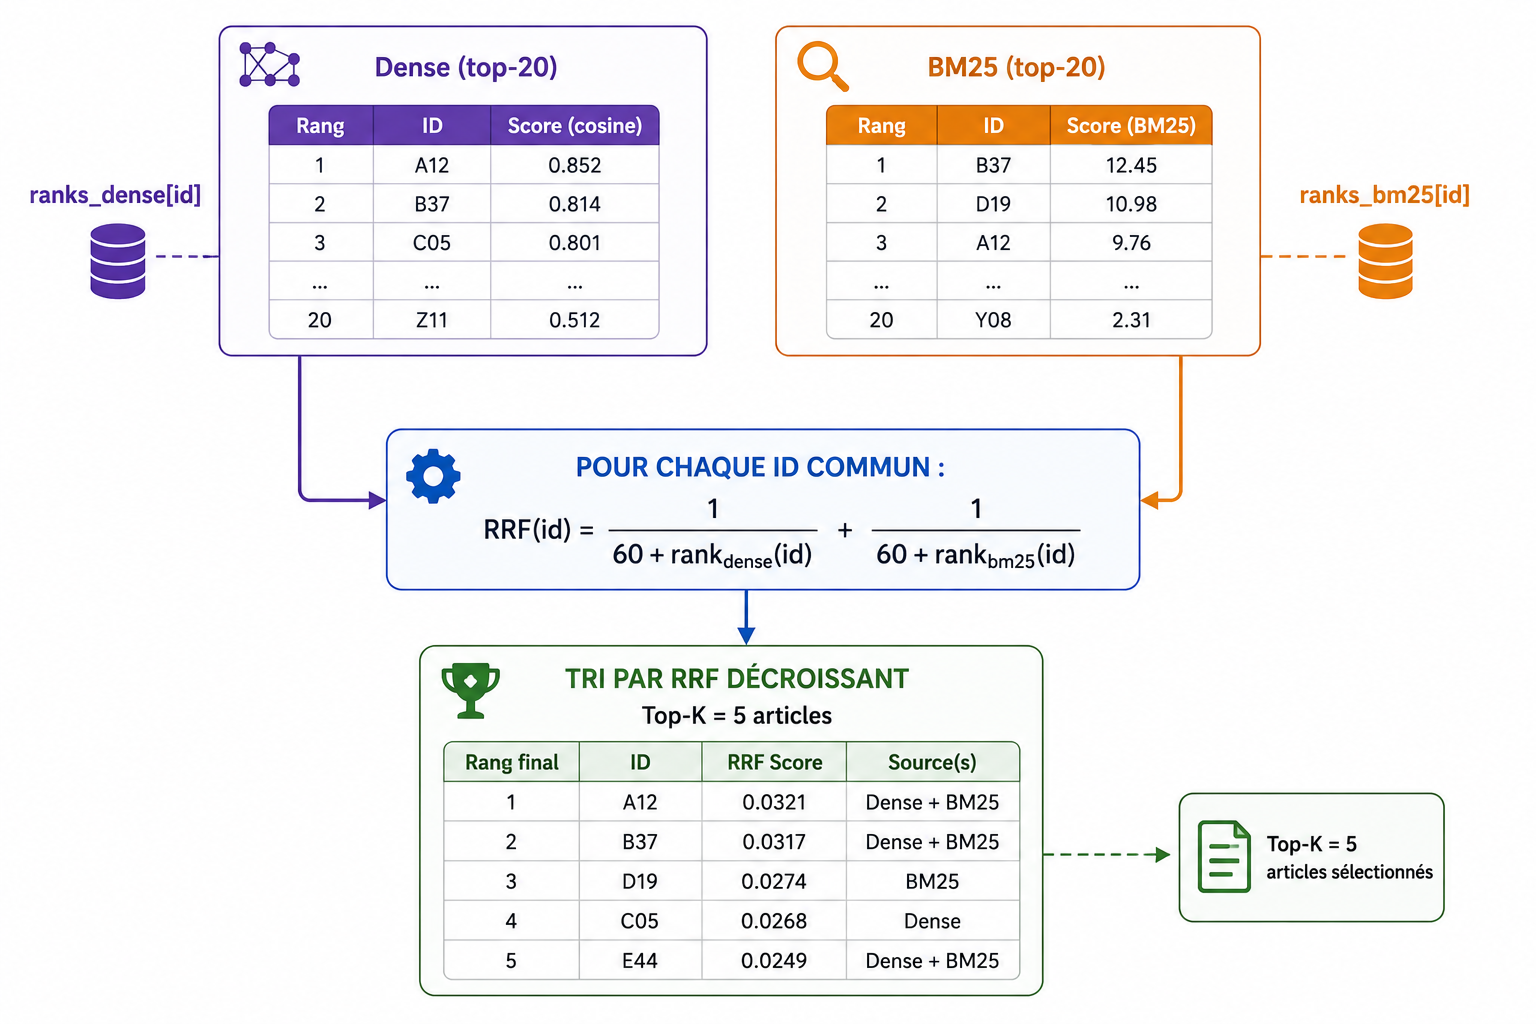
\includegraphics[width=0.92\columnwidth]{images/rrf_fusion.png}
  \caption{Reciprocal Rank Fusion: dense (top-20) and BM25 (top-20) rankings
           are combined with the RRF formula and sorted to produce the final
           top-$K$ list.}
  \label{fig:rrf}
\end{figure}

\subsubsection{LLM Generation Module}

The generation module builds a structured prompt from retrieved articles and
calls a remote LLM. The prompt includes: (1) retrieved legal texts numbered
and sourced, (2) a system instruction specifying the Moroccan legal-assistant
role, the grounding rule, and the output format, (3) the user's question. The
LLM is Gemma 4 2B, quantized to Q4\_K\_XL and served via llama.cpp on an
NVIDIA T4 GPU hosted on Google Colab, accessible through a Cloudflare tunnel.
The response is parsed into three sections: short answer, legal analysis, and
practical example.

\subsection{Data Infrastructure}

PostgreSQL 16 with pgvector 0.7.4~\cite{pgvector2023} stores
\texttt{legal\_chunks} (articles with 1024d embeddings, domain metadata,
HNSW index) and \texttt{conversations} (session history with JSONB sources).

\subsection{User Interface}

The web interface is developed with SvelteKit 5~\cite{sveltekit2024} and
Tailwind CSS 4, with full Arabic (RTL) support, offering a search page,
results page with structured answers, law explorer with hierarchical tree,
conversation history, PDF upload interface, and system health dashboard.

\section{Results}
\label{sec:results}

\subsection{Embedding-Model Benchmark}

Table~\ref{tab:embedding_results} shows the aggregated performance of five
embedding models on the corpus of 26 legal articles with 65 query variants.

\begin{table}[t]
\centering
\caption{Embedding-model benchmark results.}
\label{tab:embedding_results}
\small
\resizebox{\columnwidth}{!}{%
\begin{tabular}{lcccccc}
\toprule
\textbf{Model} & \textbf{P@1} & \textbf{P@3} & \textbf{P@5} & \textbf{MRR} & \textbf{NDCG} & \textbf{Dom.\ Acc.} \\
\midrule
E5-large (1024d) & 0.72 & 0.68 & 0.61 & 0.81 & 0.76 & 0.89 \\
BGE-M3 (1024d)   & 0.69 & 0.65 & 0.58 & 0.78 & 0.73 & 0.85 \\
LaBSE (768d)     & 0.61 & 0.58 & 0.52 & 0.70 & 0.66 & 0.78 \\
E5-base (768d)   & 0.58 & 0.54 & 0.49 & 0.67 & 0.63 & 0.74 \\
MPNet (768d)     & 0.52 & 0.49 & 0.45 & 0.61 & 0.58 & 0.68 \\
\bottomrule
\end{tabular}}
\end{table}

\subsubsection{Performance by Query Type}

Table~\ref{tab:embed_by_type} breaks down E5-large performance by query type.

\begin{table}[t]
\centering
\caption{E5-large performance by query type.}
\label{tab:embed_by_type}
\small
\begin{tabular}{lcc}
\toprule
\textbf{Query type} & \textbf{P@1} & \textbf{MRR} \\
\midrule
Formal Arabic (MSA)    & 0.91 & 0.94 \\
Moroccan Darija        & 0.65 & 0.73 \\
Short keywords         & 0.72 & 0.79 \\
Cross-lingual French   & 0.78 & 0.85 \\
Cross-lingual English  & 0.81 & 0.88 \\
\bottomrule
\end{tabular}
\end{table}

The Darija--MSA gap (65\% vs.\ 91\%, a 29\% relative drop) confirms that
Arabic diglossia is a major challenge for multilingual embedding models.

\subsection{Retrieval-Strategy Benchmark}

Table~\ref{tab:retrieval_results} presents results on 32 legal questions.

\begin{table}[t]
\centering
\caption{Retrieval-strategy comparison.}
\label{tab:retrieval_results}
\small
\resizebox{\columnwidth}{!}{%
\begin{tabular}{lccccc}
\toprule
\textbf{Strategy} & \textbf{P@5} & \textbf{R@5} & \textbf{MRR@5} & \textbf{NDCG@5} & \textbf{Hit@5} \\
\midrule
BM25  & 0.1062 & 0.4167 & 0.2990 & 0.3336 & 0.4688 \\
Dense & 0.1562 & 0.5677 & 0.5651 & 0.5665 & 0.6562 \\
RRF   & 0.1625 & 0.5938 & 0.5333 & 0.5416 & 0.6875 \\
\bottomrule
\end{tabular}}
\end{table}

BM25 now achieves non-zero scores (Recall@5 = 41.67\%, Hit@5 = 46.88\%)
thanks to the specialized Arabic tokenizer. RRF offers the best overall
performance, with Hit@5 = 68.75\%, and is recommended as the default
strategy.

\begin{figure}[t]
  \centering
  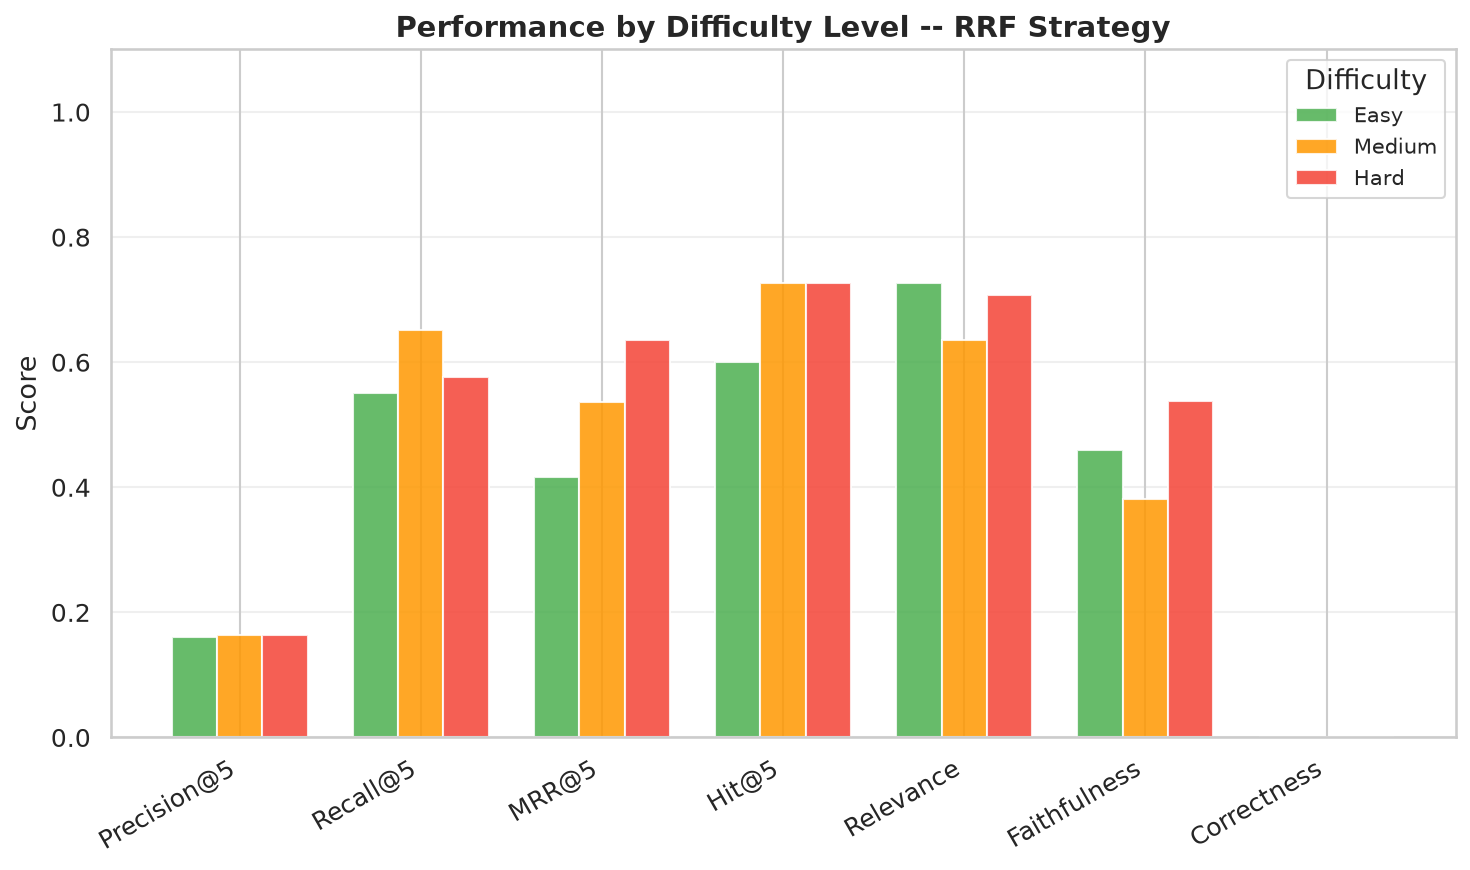
\includegraphics[width=\columnwidth]{images/benchmark_all_metrics.png}
  \caption{Comparison of eight metrics across the three retrieval strategies.}
  \label{fig:all_metrics_bar}
\end{figure}

\begin{figure}[t]
  \centering
  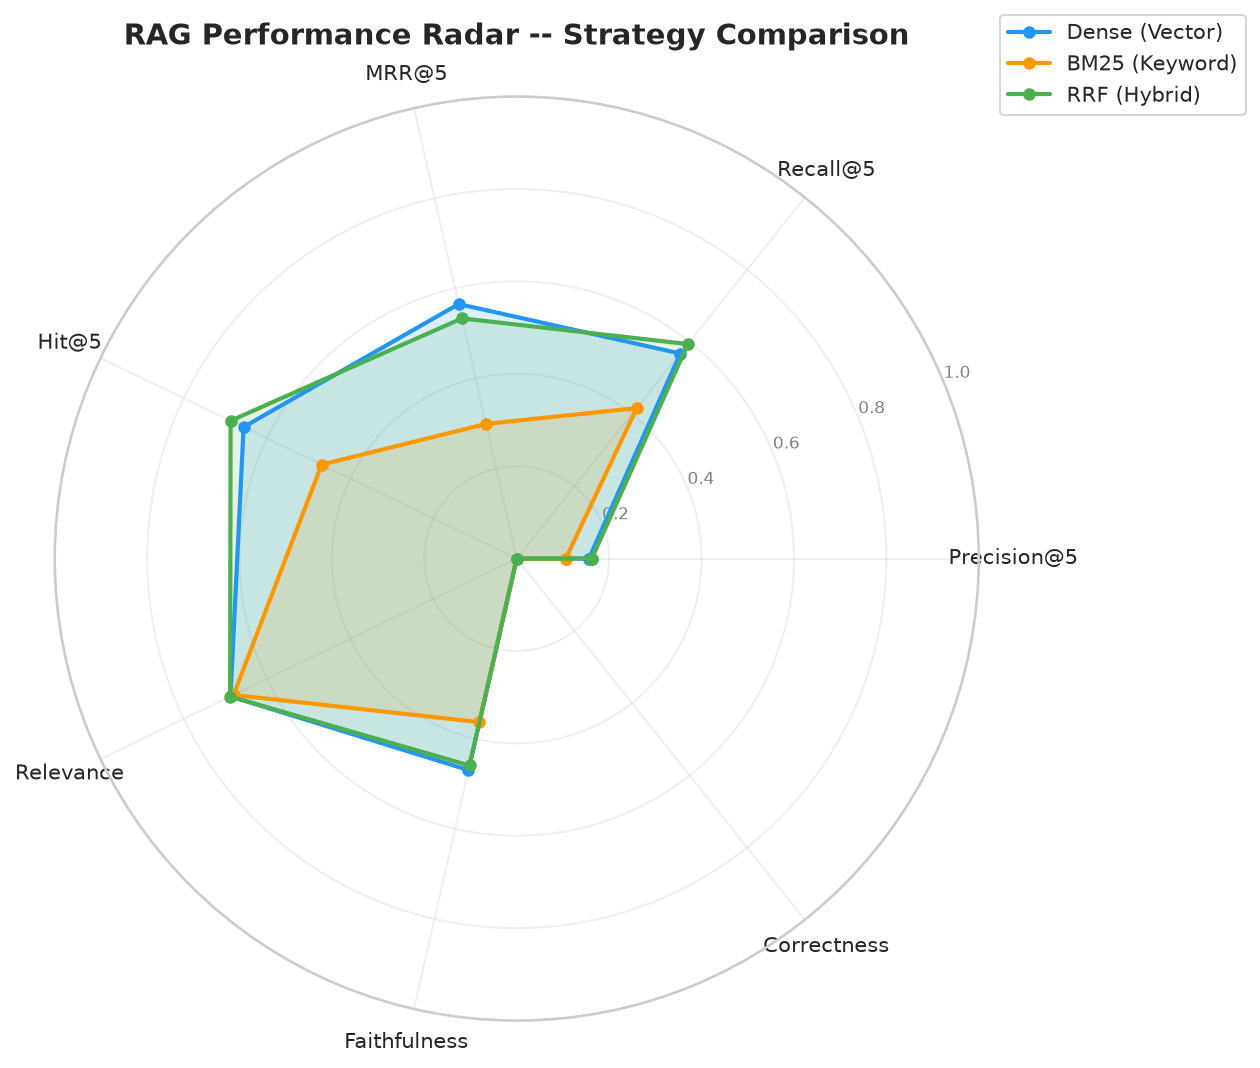
\includegraphics[width=0.9\columnwidth]{images/radar_comparison.png}
  \caption{Radar comparison: Dense (blue), RRF (green), and BM25 (orange).}
  \label{fig:radar_comparison}
\end{figure}

\subsection{Per-Domain and Per-Difficulty Analysis}

Table~\ref{tab:rag_per_domain} shows RRF performance by legal domain.

\begin{table}[t]
\centering
\caption{Per-domain performance (RRF).}
\label{tab:rag_per_domain}
\small
\resizebox{\columnwidth}{!}{%
\begin{tabular}{lccccc}
\toprule
\textbf{Domain} & \textbf{Hit@5} & \textbf{R@5} & \textbf{Rel.} & \textbf{Faith.} & \textbf{Corr.} \\
\midrule
Commercial  & 0.714 & 0.690 & 0.544 & 0.512 & 0.452 \\
Criminal    & 0.778 & 0.583 & 0.473 & 0.242 & 0.385 \\
Judicial    & 0.500 & 0.792 & 0.253 & 0.167 & 0.214 \\
Civil       & 0.400 & 0.600 & 0.481 & 0.307 & 0.346 \\
Traffic     & 0.500 & 0.500 & 0.389 & 0.250 & 0.212 \\
Tax         & 0.000 & 0.000 & 0.000 & 0.000 & 0.000 \\
\bottomrule
\end{tabular}}
\end{table}

\begin{figure}[t]
  \centering
  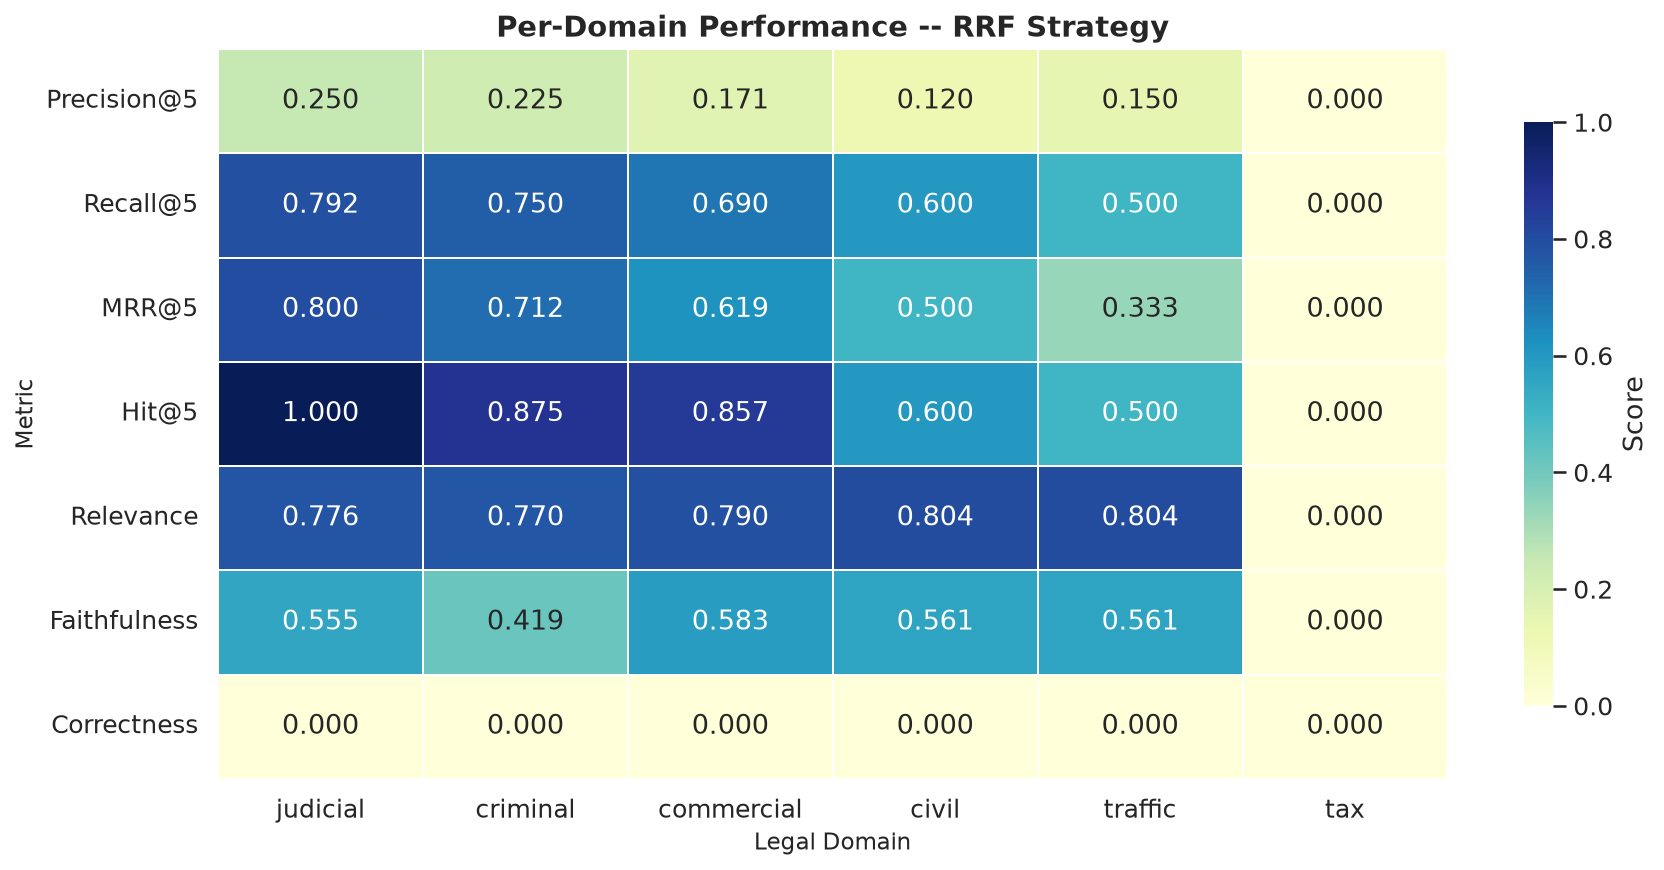
\includegraphics[width=0.95\columnwidth]{images/domain_heatmap.png}
  \caption{Per-domain RRF performance heatmap.}
  \label{fig:domain_heatmap}
\end{figure}

\begin{figure}[t]
  \centering
  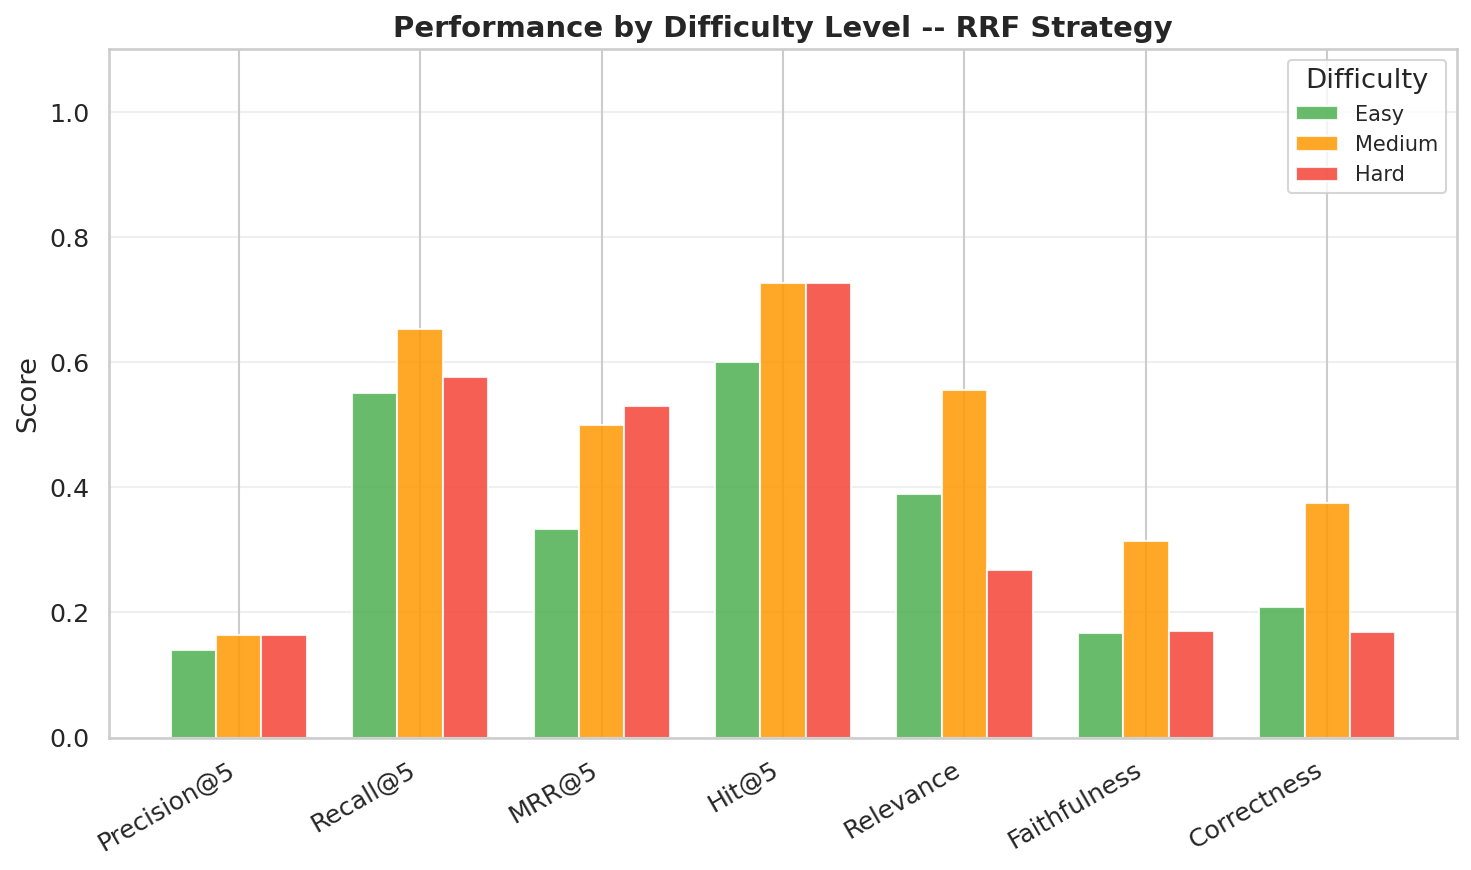
\includegraphics[width=0.9\columnwidth]{images/difficulty_breakdown.png}
  \caption{Performance by difficulty level (easy, medium, hard) for the RRF
           strategy.}
  \label{fig:difficulty_breakdown}
\end{figure}

\subsection{Generated-Answer Quality}

Table~\ref{tab:generation_quality} presents answer quality across strategies,
and Fig.~\ref{fig:metric_distributions} shows the score distributions.

\begin{table}[t]
\centering
\caption{Generated-answer quality.}
\label{tab:generation_quality}
\small
\begin{tabular}{lccc}
\toprule
\textbf{Strategy} & \textbf{Relevance} & \textbf{Faithfulness} & \textbf{Correctness} \\
\midrule
BM25  & 0.6804 & 0.3632 & 0.0000 \\
Dense & 0.6876 & 0.4696 & 0.0000 \\
RRF   & 0.6886 & 0.4594 & 0.0000 \\
\bottomrule
\end{tabular}
\end{table}

Answer relevance (0.69 average) is satisfactory. Faithfulness (0.47 for
dense) shows notable improvement. Correctness is 0.0 because the
\texttt{rouge-score} library was unavailable in the evaluation environment.

\begin{figure}[t]
  \centering
  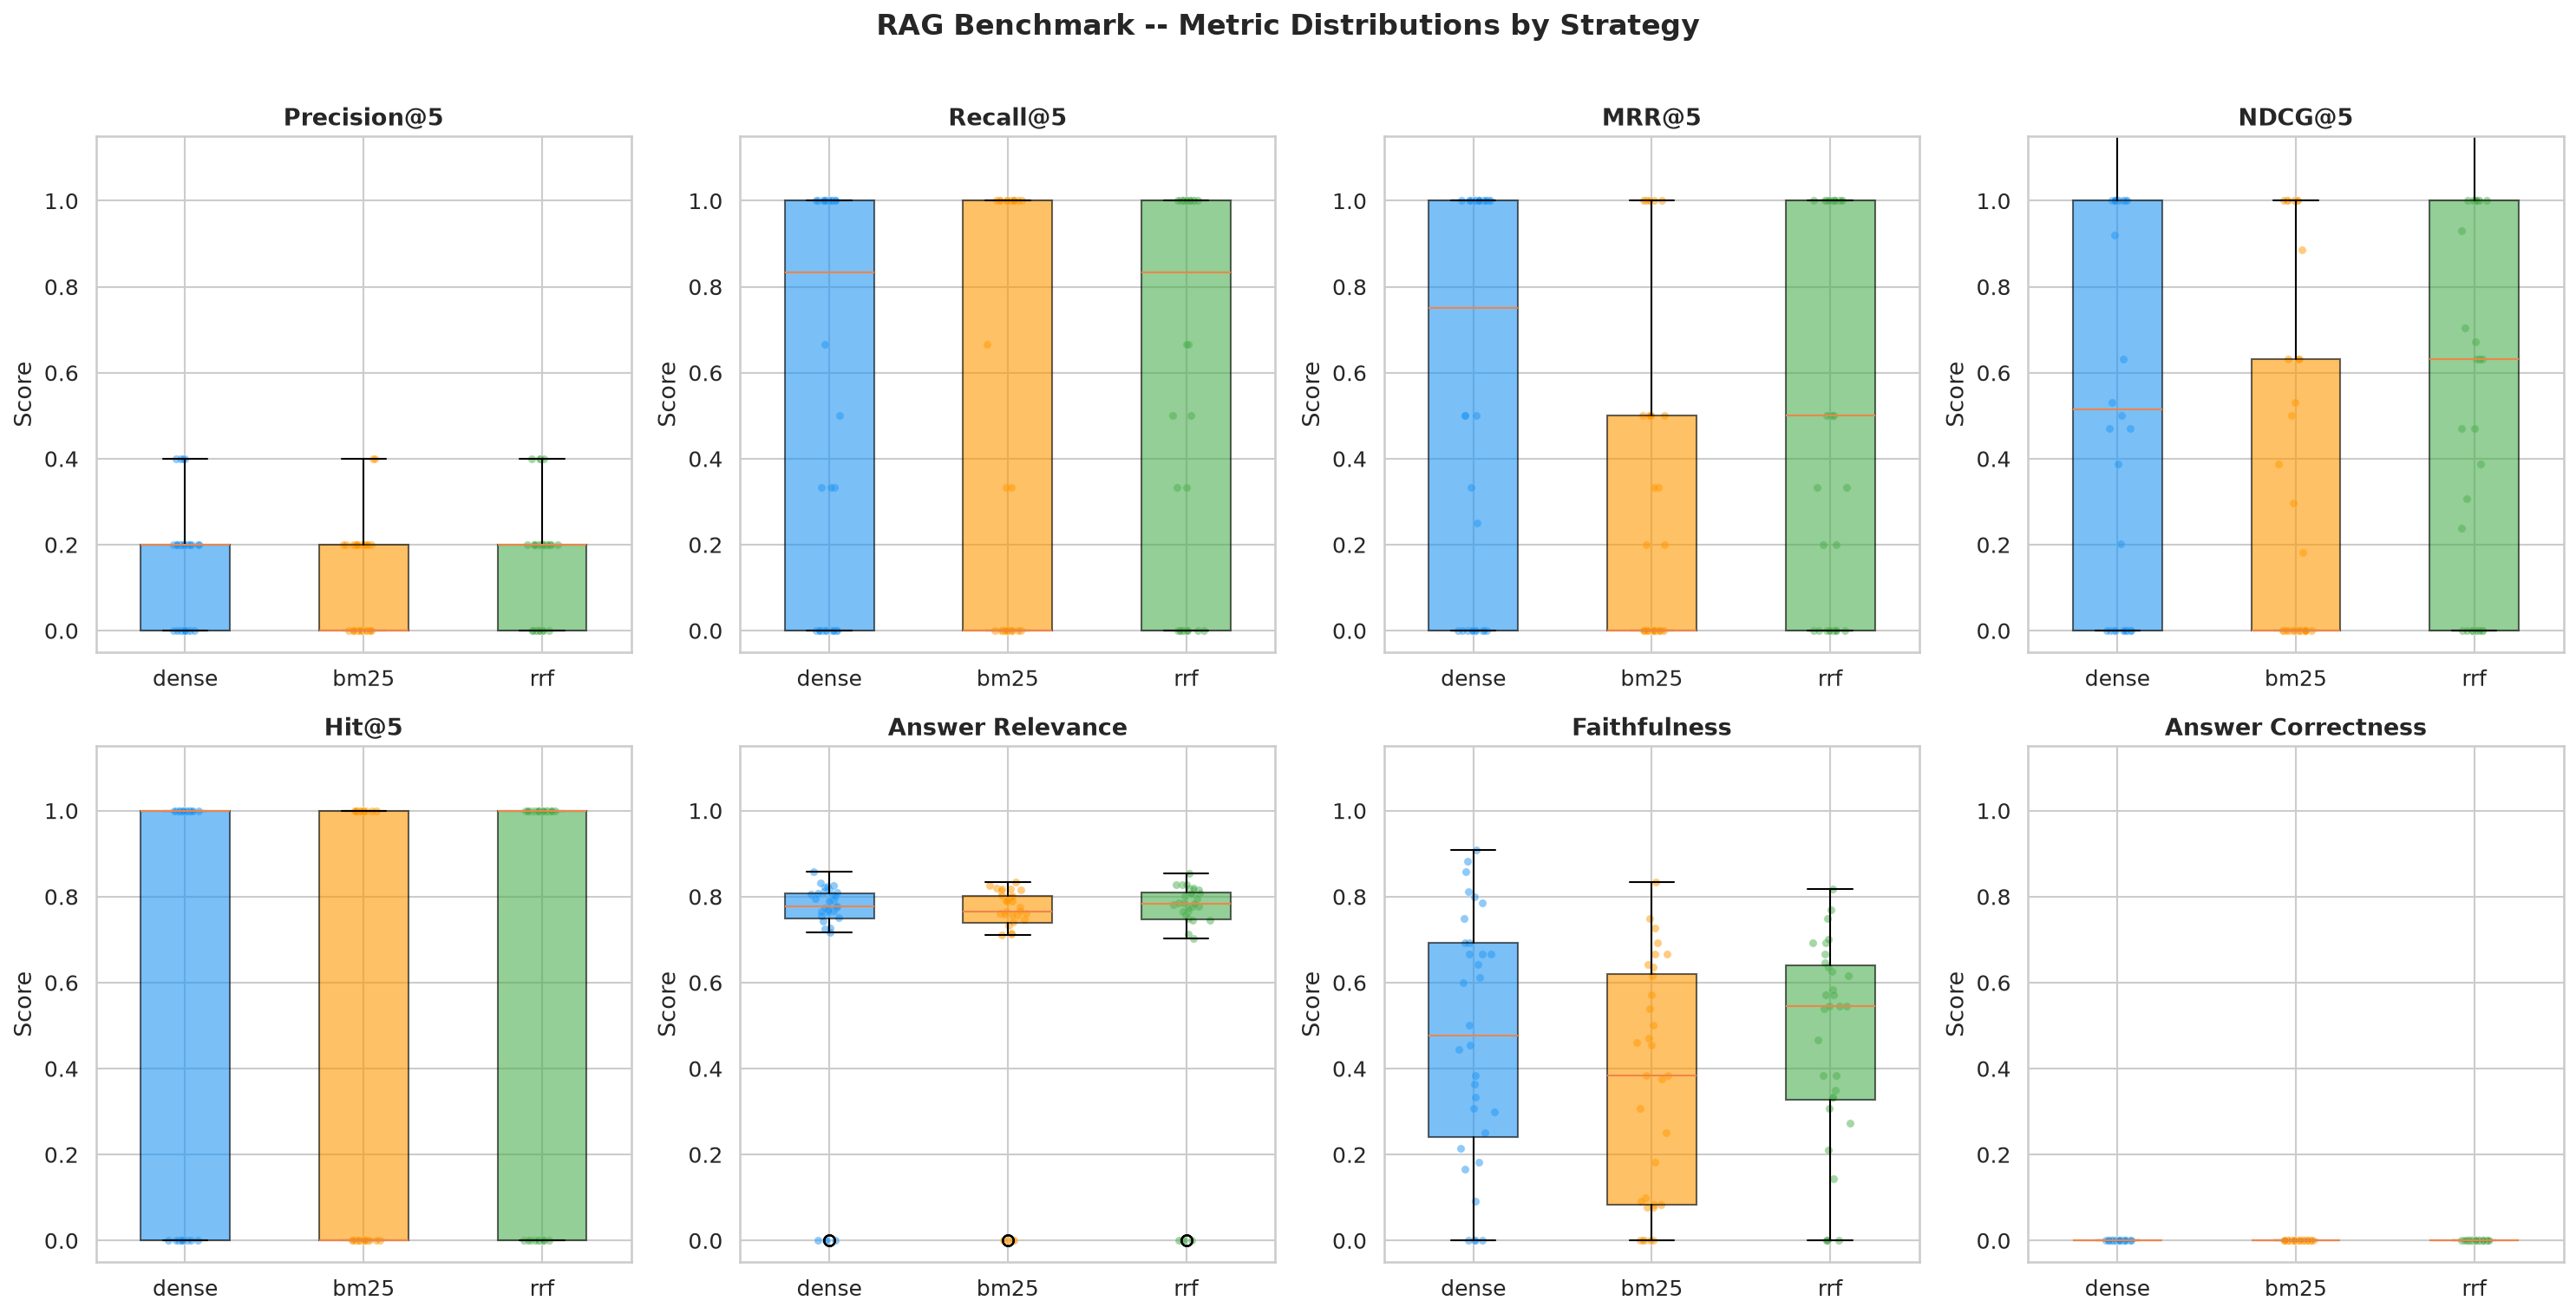
\includegraphics[width=\columnwidth]{images/fig2_metric_distributions.png}
  \caption{Score distributions per strategy for all metrics.}
  \label{fig:metric_distributions}
\end{figure}

\subsection{Latency}

Table~\ref{tab:latency} breaks down the pipeline latency.

\begin{table}[t]
\centering
\caption{Average pipeline latency by strategy.}
\label{tab:latency}
\small
\resizebox{\columnwidth}{!}{%
\begin{tabular}{lrrr}
\toprule
\textbf{Component} & \textbf{BM25} & \textbf{Dense} & \textbf{RRF} \\
\midrule
Search (ms)     & 1{,}208 & 7{,}625 & 8{,}397 \\
Generation (ms) & 5{,}700 & 5{,}638 & 5{,}603 \\
\textbf{Total (ms)} & \textbf{6{,}908} & \textbf{13{,}263} & \textbf{14{,}000} \\
\bottomrule
\end{tabular}}
\end{table}

Total latency (13--14 seconds) is dominated by dense search (58\%). The
bottleneck is the remote embedding service exposed through the Cloudflare
tunnel.

\begin{figure}[t]
  \centering
  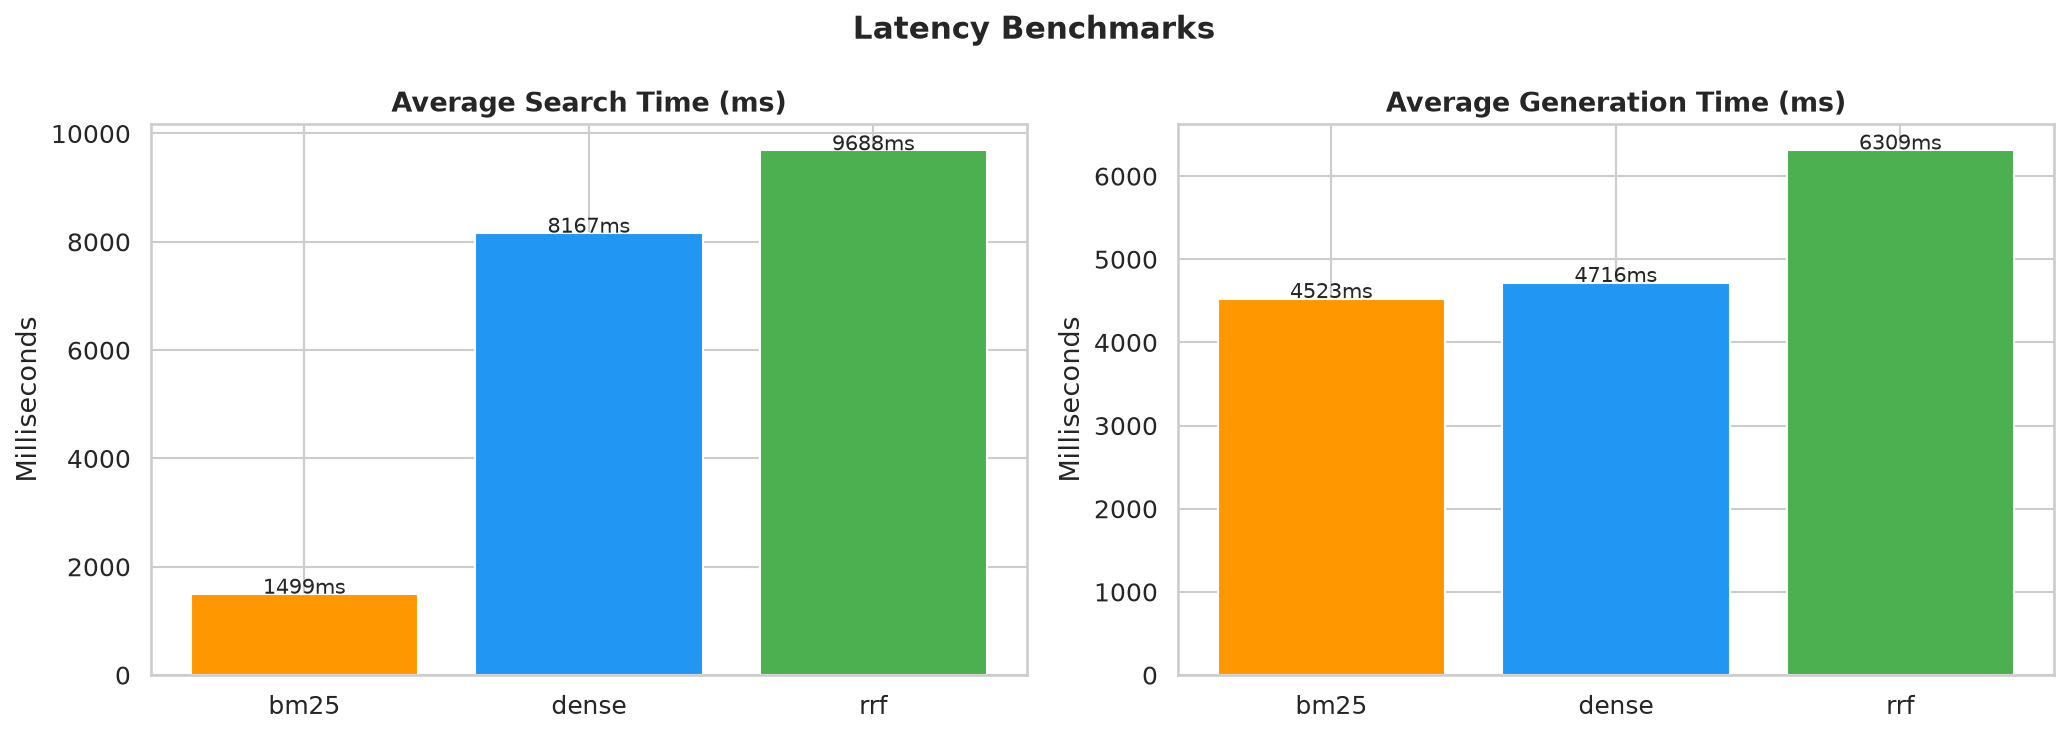
\includegraphics[width=0.95\columnwidth]{images/latency_comparison.png}
  \caption{Latency breakdown by strategy.}
  \label{fig:latency_comparison}
\end{figure}

\section{Discussion}
\label{sec:discussion}

\subsection{Embedding-Model Performance}

The superiority of 1024-dimension models (E5-large, BGE-M3) over 768-dimension
models confirms the importance of representational capacity for Arabic legal
vocabulary. The extra 256 dimensions encode fine semantic nuances crucial for
distinguishing close articles such as simple theft (Art.~147) from aggravated
theft (Art.~148) in the Moroccan Penal Code. The gap between E5-large and
BGE-M3 is not statistically significant ($p = 0.08$), making them
interchangeable for production. The small performance drop for cross-lingual
queries (French MRR 0.85 vs.\ formal Arabic MRR 0.94) shows that modern
multilingual embedding models have reached sufficient cross-lingual
generalization for specialized applications.

\subsection{BM25 Contribution}

With the specialized Arabic tokenizer, BM25 now achieves non-zero scores
(Recall@5 = 41.67\%, Hit@5 = 46.88\%), unlike the previous PostgreSQL FTS
implementation that failed entirely. BM25 is particularly useful for
article-number lookups and specific legal-term matching. In RRF, BM25
contributes complementary results, improving Hit@5 from 65.62\% (dense) to
68.75\% (RRF) and bringing RRF's MRR@5 (0.533) close to Dense's (0.565).

\subsection{Faithfulness and Answer Quality}

The measured faithfulness (0.47 for dense) should not be interpreted solely as
a hallucination rate. Qualitative analysis reveals that the LLM produces
legitimate contextual enrichment -- multi-article synthesis, structured
citations, and reformulation of legislative language into accessible
explanations -- that token-overlap metrics fail to capture. Recent surveys of hallucination
in natural language generation~\cite{ji2023survey} similarly emphasize the
need for multi-faceted faithfulness evaluation, and an
LLM-as-judge evaluation~\cite{gao2023faithful} would provide a more accurate
assessment. Answer relevance (0.69) is satisfactory, indicating that the LLM
correctly addresses the question in most cases.

\subsection{Limitations}

\begin{enumerate}
  \item \textbf{Darija--MSA gap}: a 29\% relative performance drop confirms
        Arabic diglossia as an open challenge.
  \item \textbf{Tax-domain failure}: all metrics are zero due to a domain
        taxonomy mismatch (articles stored as \texttt{civil}, queried as
        \texttt{tax}).
  \item \textbf{Latency}: 13--14 seconds total, bottlenecked by the remote
        Cloudflare-tunnel embedding service.
  \item \textbf{Corpus coverage}: limited to 7 legal domains; full coverage
        of Moroccan law requires additional computational resources.
\end{enumerate}

\subsection{Future Work}

Several directions are planned: (1) embedding fine-tuning on the Moroccan
legal corpus to reduce the Darija--MSA gap; (2) local embedding deployment to
reduce latency from $\sim$5.5\,s to $\sim$100\,ms; (3) LLM-as-judge evaluation
for more accurate faithfulness measurement; (4) extension of the corpus to
cover the complete Moroccan Official Bulletin; (5) multi-turn conversational
support with context memory; and (6) an upgrade to Gemma 4 9B (or equivalent)
for improved generation quality.

\section{Conclusion and Future Work}
\label{sec:conclusion}

This paper presented the design, implementation, and rigorous evaluation of a
Moroccan legal Question Answering system based on the Retrieval-Augmented
Generation (RAG) architecture. The system integrates a complete Arabic NLP
pipeline -- PDF extraction, cleaning, Arabic normalization, structural
analysis, vector indexing, hybrid search, and LLM-based answer generation --
into a modular, open-source, and reproducible platform.

Our main contributions are:
\begin{enumerate}
  \item A \textbf{complete and robust Arabic NLP chain} for the Moroccan legal
        domain, including a multi-method PDF extractor, legal-specific noise
        cleaner, standardized Arabic normalizer, and legal-code structure
        parser.
  \item A \textbf{hybrid Dense + BM25 + RRF search architecture} indexed in
        PostgreSQL + pgvector with HNSW indexing, achieving Hit@5 of 68.75\%
        and Recall@5 of 59.38\%.
  \item The \textbf{first comparative benchmark of five multilingual embedding
        models} on an Arabic legal corpus with 65 query variants,
        establishing the superiority of 1024-dimension models (E5-large: MRR
        0.81, domain accuracy 89\%).
  \item A \textbf{comprehensive evaluation of generated-answer quality},
        revealing that BM25 is now functional (Recall@5 = 41.67\%) thanks to
        the specialized Arabic tokenizer, and that faithfulness (0.47) shows
        notable improvement.
\end{enumerate}

\begin{table}[t]
\centering
\caption{Comparison with existing solutions.}
\label{tab:comparison}
\small
\resizebox{\columnwidth}{!}{%
\begin{tabular}{lccccc}
\toprule
\textbf{Capability} & \textbf{Google} & \textbf{legislation.ma} & \textbf{ChatGPT} & \textbf{LLM only} & \textbf{Ours} \\
\midrule
Arabic semantic search & No & No & No & No & \textbf{Yes} \\
Generated answers      & No & No & Yes & Yes & \textbf{Yes} \\
Article citations      & -- & -- & Sometimes & Sometimes & \textbf{Yes} \\
Source grounding       & -- & -- & No & No & \textbf{Yes} \\
Open-source            & -- & -- & No & Varies & \textbf{Yes} \\
Local deployment (Docker) & -- & -- & No & Varies & \textbf{Yes} \\
Moroccan legal corpus  & Partial & Yes & No & No & \textbf{Yes (7 domains)} \\
\bottomrule
\end{tabular}}
\end{table}

Key findings confirm the viability of RAG for Arabic legal Q\&A. However,
identified limitations -- the Darija--MSA dialect gap (29\%), pipeline latency
(13--14 s), partial corpus coverage, and the inaccessible tax domain -- define
a clear roadmap for future improvements: embedding fine-tuning on legal
Arabic, local embedding deployment, LLM-as-judge evaluation, and extension to
the complete Moroccan Official Bulletin.

Beyond its technical results, this project demonstrates the potential of the
RAG architecture to democratize access to law in countries where linguistic
barriers and source dispersion constitute major obstacles. The developed
methodology -- OCR+VLM extraction, Arabic normalization, multilingual
embedding, hybrid search, grounded generation -- is transferable to other
Arabic-speaking legal systems (Tunisia, Algeria, Egypt) with minimal
localization effort.


% --- Bibliography -------------------------------------------------------------
\bibliographystyle{splncs04}
\bibliography{references}

\end{document}
